\documentclass[8pt,aspectratio=169]{beamer}
\usetheme{Boadilla}

\usepackage{hyperref}
\usepackage{graphicx}
\usepackage{subfig}
\usepackage{amsmath,amssymb,physics}

\graphicspath{ {img_talk/} }

\usepackage{tikz}

% Set beamer color info
\definecolor{BOrange}{RGB}{191,87,0}
\setbeamercolor{title}{fg=black}
\setbeamercolor{frametitle}{fg=black}
\setbeamercolor{structure}{fg=BOrange}


%Stolen from https://tex.stackexchange.com/questions/388344/beamer-adding-some-text-in-subsection-title-page
\setbeamertemplate{section page}
{
    \begingroup
    \begin{beamercolorbox}[sep=10pt,center,rounded=true,shadow=true]{section title}
        \usebeamerfont{section title}\insertsection\par
    \end{beamercolorbox}
    \endgroup
}

\title{Holographic Complexity}
\author{Josiah Couch}
\institute{University of Texas at Austin}
%\institute{At Oklahoma State University}
\date{14 April 2021}



\begin{document}

\begin{frame}
\titlepage\end{frame}

\begin{frame}
\frametitle{Outline}
\tableofcontents[]
\end{frame}

\section{Introduction}
\begin{frame}
\sectionpage
\end{frame}

\subsection{AdS/CFT and Holography}

\begin{frame}
\frametitle{The AdS/CFT correspondence}

\onslide<1->{
\begin{minipage}[t]{0.48\linewidth}

\begin{itemize}

\item \onslide<2->{'bulk' gravity theory in $d+1$ dimensional  asymptotically AdS spacetime $\leftrightarrow$ 'boundary' $d$ dimensional conformal field theory}

\hfill

\item \onslide<3->{boundary strong coupling $\leftrightarrow$ bulk weak coupling}

\hfill

\item \onslide<4->{large $N$ boundary $\leftrightarrow$ classical bulk}

\hfill

\item \onslide<5->{CFT operators $\leftrightarrow$ bulk fields}

\hfill

\item \onslide<6>{boundary thermal state $\leftrightarrow$ black hole (above Hawking-Page transition)}

\end{itemize}

\end{minipage}
%
\hfill
%
\begin{minipage}[t]{0.48\linewidth}

\only<1>{
\begin{figure}
    \begin{center}
    
        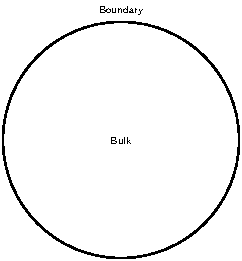
\includegraphics[scale=1]{adscft0.pdf}    
    
    \end{center}
    \caption{The AdS/CFT Correspondence}
    \label{fig:adscft}
\end{figure}
}

\only<2>{
\begin{figure}
    \begin{center}
    
        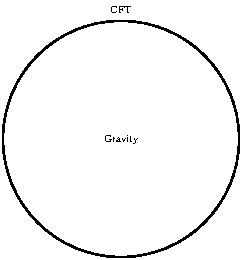
\includegraphics[scale=1]{adscft.pdf}    
    
    \end{center}
    \caption{The AdS/CFT Correspondence}
\end{figure}
}

\only<3>{
\begin{figure}
    \begin{center}
    
        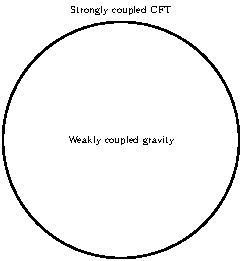
\includegraphics[scale=1]{adscft2.pdf}    
    
    \end{center}
    \caption{The AdS/CFT Correspondence}
\end{figure}
}

\only<4>{
\begin{figure}
    \begin{center}
    
        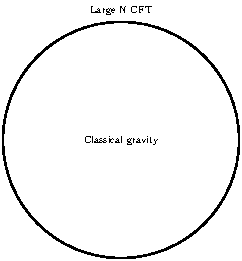
\includegraphics[scale=1]{adscft3.pdf}    
    
    \end{center}
    \caption{The AdS/CFT Correspondence}
\end{figure}
}

\only<5>{
\begin{figure}
    \begin{center}
    
        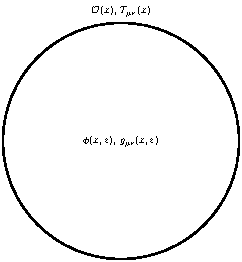
\includegraphics[scale=1]{adscft4.pdf}    
    
    \end{center}
    \caption{The AdS/CFT Correspondence}
\end{figure}
}

\only<6>{
\begin{figure}
    \begin{center}
    
        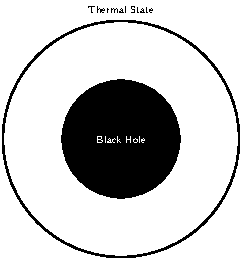
\includegraphics[scale=1]{adscftBH.pdf}    
    
    \end{center}
    \caption{The AdS/CFT Correspondence}
\end{figure}
}

\end{minipage}
}

\end{frame}

\begin{frame}
\frametitle{Entanglement Entropy}

\onslide<1->{Ryu-Tagayanagi (RT) prescription:

\begin{minipage}[t]{0.55\linewidth}

\begin{itemize}

\item \onslide<2->{Consider a spatial slice of our AdS spacetime}

\item \onslide<3->{On this spatial slice, specify a boundary region $A$, whose entanglement entropy we want to compute.} 

\item \onslide<4->{Consider the surface of minimal area whose boundary intersects that of our region A. We will call this the RT surface for $A$}

\item \onslide<5->{The entanglement entropy of $A$ is then the area of the RT surface over $4 G$.}

\item \onslide<6->{The causal development of the spatial region bounded by the RT surface is called the \textit{entanglement wedge}}

\item \onslide<7->{The mixed state on $A$ is dual to the entanglement wedge of $A$.}

\end{itemize}

\end{minipage}\hfill
%
\begin{minipage}[t]{0.44\linewidth}

\only<1-2>{
\begin{figure}
    \begin{center}
    
        
\includegraphics[scale=1]{RT0}  
    
    \end{center}
    \caption{The Ryu-Takayanagi Prescription}
    \label{fig:RT0}
\end{figure}
}

\only<3>{
\begin{figure}
    \begin{center}
    
        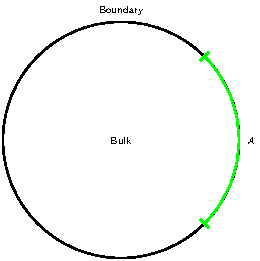
\includegraphics[scale=1]{RT1}  
    
    \end{center}
    \caption{The Ryu-Takayanagi Prescription}
    \label{fig:RT1}
\end{figure}
}

\only<4->{
\begin{figure}
    \begin{center}
    
        
\includegraphics[scale=1]{RT}  
    
    \end{center}
    \caption{The Ryu-Takayanagi Prescription}
    \label{fig:RT}
\end{figure}
}

\end{minipage}
}

\onslide<8>{By considering all possible subregions and their respective entanglement entropies, we may hope to reconstruct the dual bulk geometry from field theory data.}

\end{frame}
\subsection{Holographic Complexity}

\begin{frame}
\frametitle{Holographic Complexity}

\onslide<1->{
There are some puzzling aspects to the geometry behind the horizon.

\begin{minipage}[t]{0.55\linewidth}

\begin{itemize}

\item \onslide<2->{No region defined entirely on the left or right side is sensitive to this part of the geometry}

\item \onslide<3->{The volume behind the horizon on a spatial slice continues growing long past the thermal time.}

\end{itemize}

\onslide<4->{To resolve these issues, Leonard Susskind proposed that the geometry behind the horizon is dual to the \textit{quantum circuit complexity} of the dual state.}

\begin{itemize}

\item \onslide<5->{Specifically, Susskind proposed that the complexity of boundary state is dual to the volume of a maximal spatial slice of the bulk. (Complexity = volume) \cite{Susskind:2014rva}}

\item \onslide<6->{Most of the increase in such a slice with time occurs behind the horizon.}

\item \onslide<7->{Like the volume, the complexity of the state obtained from the TFD state by unitary time evolution is expected to increase long past the thermalization time}

\item \onslide<8>{Later, 'complexity = action' (CA) was proposed as an alternative to CV, which states that complexity is dual to the action of the WDW patch}

\end{itemize}

\end{minipage}\hfill
%
\begin{minipage}[t]{0.44\linewidth}

\only<1-4>{
\begin{figure}
    \begin{center}
    
        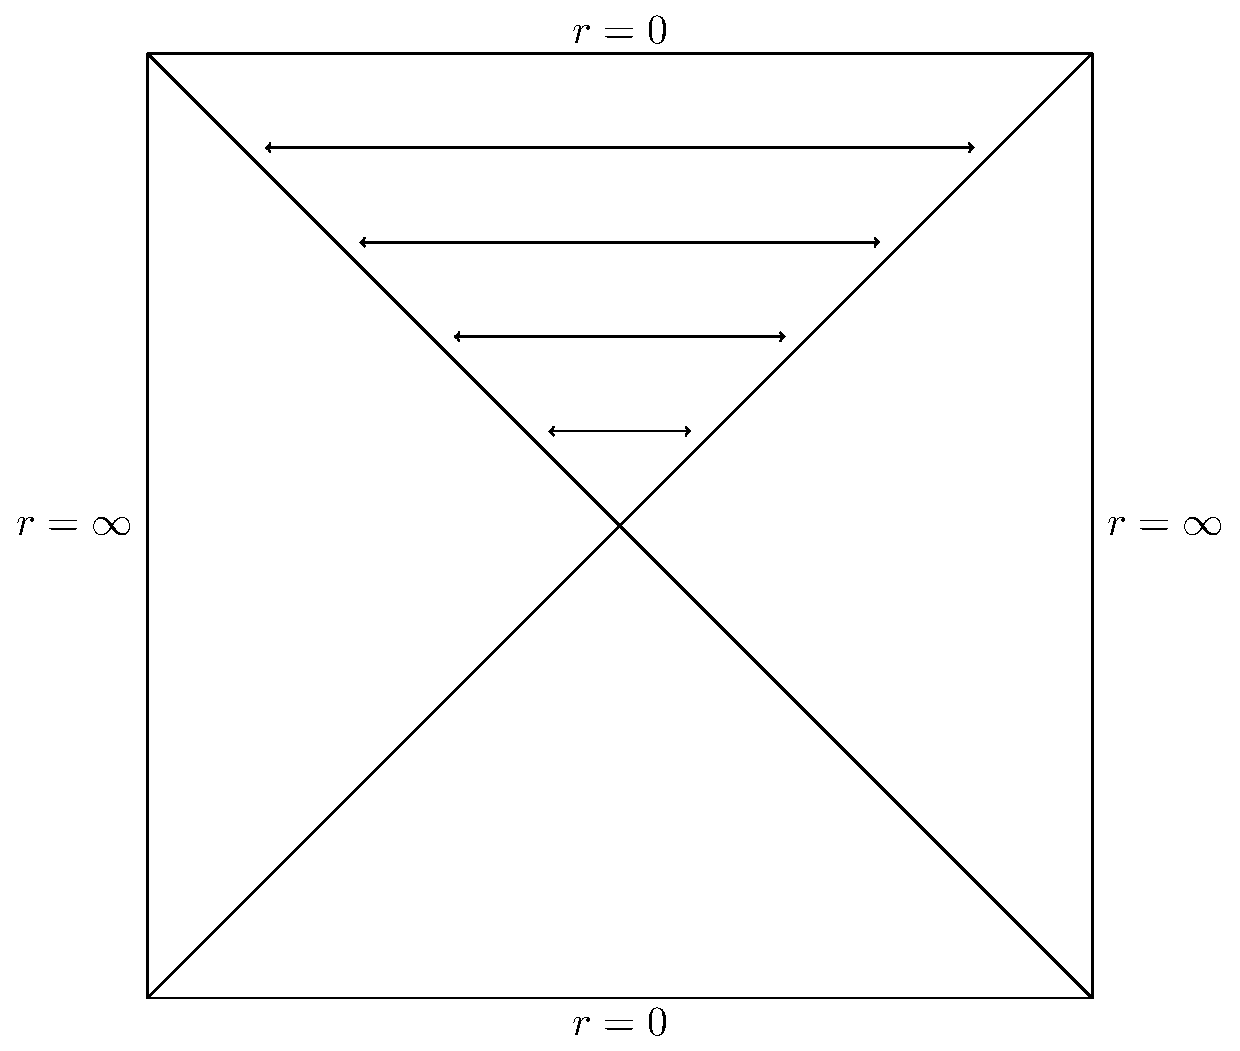
\includegraphics[scale=0.3]{WormholeGrowth}     
    
    \end{center}
    \caption{Growth of the wormhole}
    \label{fig:WomholeGrowth}
\end{figure}
}

\only<5->{
\begin{figure}
    \begin{center}
    
        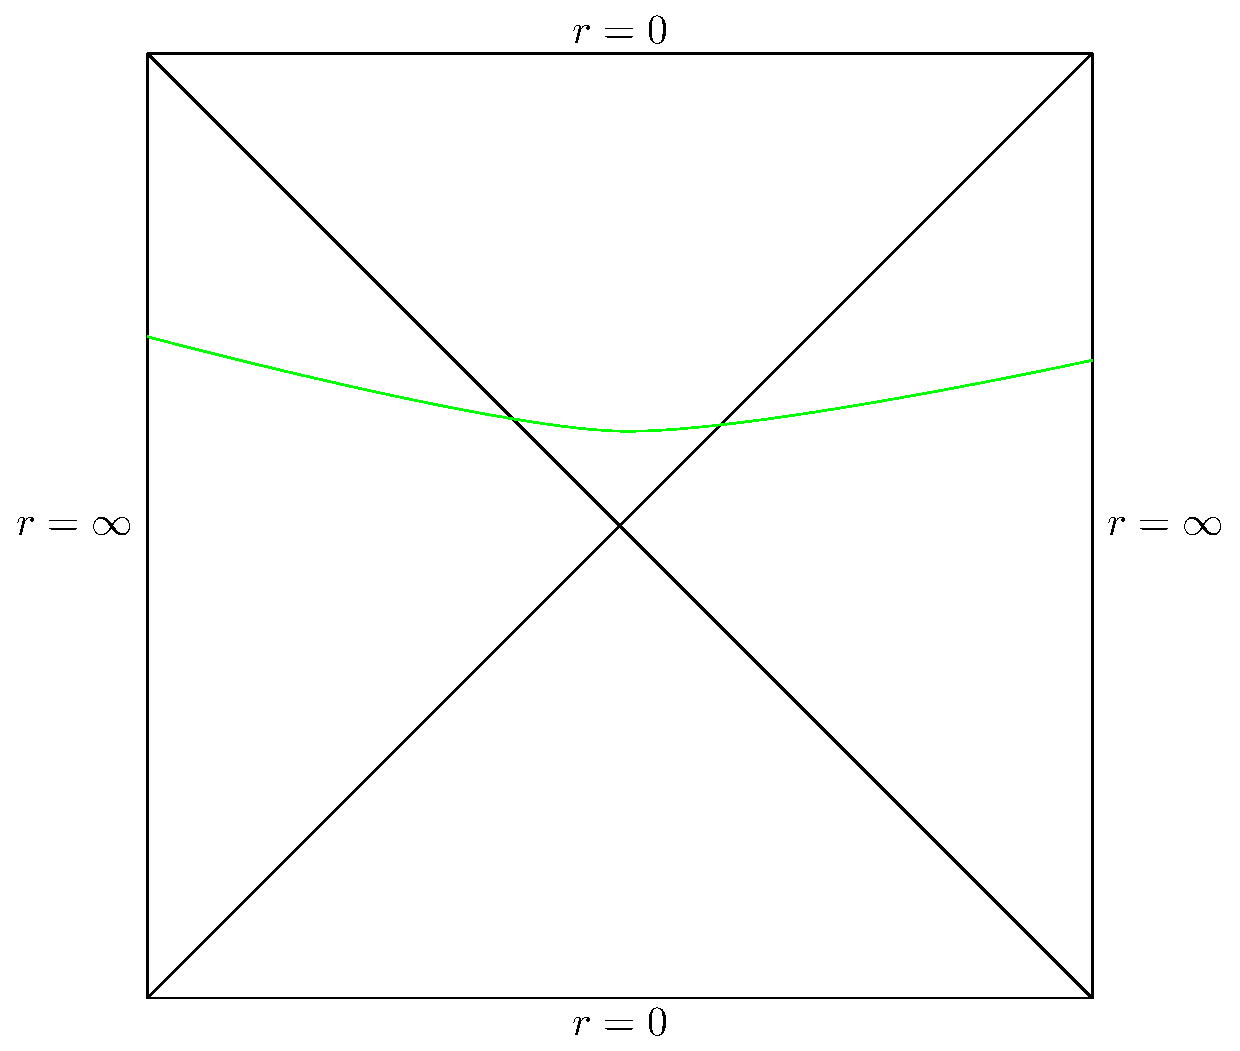
\includegraphics[scale=0.3]{CV}     
    
    \end{center}
    \caption{Maximal Volume Slice}
    \label{fig:CV}
\end{figure}
}

\end{minipage}
}

\end{frame} 

\begin{frame}
\frametitle{Quantum Circuit Complexity}

What is circuit complexity?

\hfill

\begin{itemize}

\item \onslide<2->{Gate: One of a chosen collection of unitary operators}

\hfill

\item \onslide<3->{Circuit: A (formal) product of some number of gates}

\hfill

\item \onslide<4->{Universal gate set: A set of gates such that every unitary can be approximated by a circuit (to within $\epsilon$)}

\hfill

\item \onslide<5->{Complexity of a circuit: 
%
\begin{equation}
\mathcal{C}\left(Q\right) = \text{ number of gates in } Q
\end{equation}
}

\hfill

\item \onslide<6->{Complexity of a unitary: 
%
\begin{equation}
\mathcal{C}\left(U\right) = \min_{Q: ||U-Q||\leq \epsilon} \mathcal{C}(Q)
\end{equation}
}

\hfill

\item \onslide<7>{Complexity of a state (relative to a reference): 
%
\begin{equation}
\mathcal{C}\left(\ket{\psi}\right) = \min_{U: U\ket{r} = \ket{\psi}} \mathcal{C}(U)
\end{equation}
}

\end{itemize}

\end{frame}


\begin{frame}
\frametitle{The WDW patch}

\onslide<1->{
\begin{minipage}[t]{0.45\linewidth}

\begin{itemize}

\item \onslide<1->{The WDW patch is defined by a spatial slice of the boundary.} 

\item \onslide<2->{For a two-sided black hole, this can be given by a left time $t_L$ and a right time $t_R$.}

\item \onslide<3->{The WDW patch is then defined as the union of all spatial slices which meet the left boundary at $t_L$ and the right boundary at $t_R$, along with the null boundary of this region.}

\item \onslide<4->{The action of this patch diverges at the boundary, so we will regularize by a cutoff}

\item \onslide<5->{Often, we will be interested in the rate of change of the action, as $t_L$ increases.}

\item \onslide<6->{This may be computed by subtracting the actions of two WDW patches, whose left time is separated by $\delta t$, and then taking the limit where $\delta t \rightarrow 0$.}

\item \onslide<7>{This difference of actions decomposes to the difference of two bulk pieces, a piece from the spacelike boundary of a near singularity cutoff, and two codimension two contributions from the past corners of the patches.}

\end{itemize}

\end{minipage}\hfill
%
\begin{minipage}[t]{0.54\linewidth}

\only<1-2>{
\begin{figure}
    \begin{center}
    
        
\includegraphics[scale=0.4]{WDW0.pdf}    
    
    \end{center}
    \caption{Boundary times $t_L$ and $t_R$}
    \label{fig:WDW}
\end{figure}
}

\only<3>{
\begin{figure}
    \begin{center}
    
        
\includegraphics[scale=0.4]{WDW.pdf}    
    
    \end{center}
    \caption{WDW patch for times $t_L$ and $t_R$}
    \label{fig:WDW}
\end{figure}
}

\only<4>{
\begin{figure}
    \begin{center}
    
        
\includegraphics[scale=0.4]{WDW2.pdf}    
    
    \end{center}
    \caption{Regulated WDW patch}
    \label{fig:WDW}
\end{figure}
}

\only<5->{
\begin{figure}
    \begin{center}
    
        
\includegraphics[scale=0.4]{2WDW.pdf}    
    
    \end{center}
    \caption{Regions which contribute to rate of change}
    \label{fig:WDW}
\end{figure}
}

\end{minipage}
}

\end{frame}


\begin{frame}
\frametitle{Part I recap}

\begin{itemize}

\item \onslide<1->{The AdS/CFT correspondence gives us a window into strongly coupled field theory and quantum gravity.}

\hfill

\item \onslide<2->{While AdS/CFT should allow us to reconstruct the interior of a black hole from boundary data, it is not clear how to do that.}

\hfill

\item \onslide<3->{The holographic complexity conjectures suggest a relation between certain features that capture aspects of the geometry behind the horizon and the circuit complexity of the dual state.}

\hfill

\item \onslide<4->{These conjectures come in two versions, 'complexity = action' and 'complexity = volume'.}

\hfill

\item \onslide<5->{While there are qualitative arguments in favor of these conjectures, we do not have any solid demonstration that they are true.}

\end{itemize}

\end{frame}


\section{Holographic Complexity and Extended Thermodynamics}
\begin{frame}
\sectionpage
	\begin{center}
		Based on 1610.02038\\
		Work with Willy Fischler and Phuc Nguyen
	\end{center}
\end{frame}

\subsection{Extended Thermodynamics}

\begin{frame}
\frametitle{Where is PV in black hole thermodynamics?}

\begin{itemize}

\item \onslide<1->{The usual first law of black hole thermodynamics reads
\begin{equation}
d M = \frac{\kappa}{8\pi G} d A + \Omega d J + \Phi d Q
\end{equation}
} 

\hfill

\item \onslide<2->{Of course we interpret these as follows:
\begin{eqnarray}
&M \rightarrow U \\
&\kappa \rightarrow 2\pi T &A \rightarrow 4 G S \\
&\Phi \rightarrow \mu &Q \rightarrow Q \\
&\Omega \rightarrow \Omega &J\rightarrow J 
\end{eqnarray}
} 

\item \onslide<3->{Notably missing in this first law is a $PV$ work term, like the one in the first law for an ideal gas. 
} 

\item \onslide<4>{However, one can think of the cosmological constant as giving rise to a pressure according to
\begin{equation}
P = - \frac{\Lambda}{8 \pi G}
\end{equation}
} 

\end{itemize}

\end{frame}

\begin{frame}
\frametitle{Thermodynamic Volume}

\begin{itemize}

\item \onslide<1->{By varying the cosmological constant $\Lambda$, and thus the pressure $P$, one get's an extended first law of the form
\begin{equation}
d M = T d S + \Omega d J + \mu d Q + V_{th} d P
\end{equation}
} 

\item \onslide<2->{Here $V_{th}$ is defined by 
\begin{equation}
V_{th} := \left(\frac{\partial M}{\partial P} \right)_{S,Q,J}
\end{equation} 
} 

\item \onslide<3->{For 3+1 AdS-RN we have }
\begin{eqnarray}
\onslide<4->{f(r) &=& g_{tt} = \frac{1}{g_{rr}} = 1 - \frac{2 M G}{r} + \frac{Q^2}{r^2} + \frac{r^2}{L^2}}\\
\onslide<5->{f(r_+) &=& 0 \Rightarrow M = \frac{r_+}{2G}\left[1 + \frac{Q^2}{r_+^2} + \frac{r_+^2}{L^2} \right]}\\
\onslide<6->{ &=& \sqrt{\frac{S}{4\pi G}}\left[ 1 + \frac{\pi Q^2}{G S} + \frac{8 G^2 P S}{3} \right]}\\
\onslide<7>{ \Rightarrow V_{th} &=& \frac{4}{3 \sqrt{\pi}} (GS)^{\frac{3}{2}} = \boxed{\frac{4}{3} \pi r_+^3} \text{ !}}
\end{eqnarray}


\end{itemize}

\end{frame}

\begin{frame}
\frametitle{Interpretation of Thermodynamic Volume}

\begin{itemize}

\item \onslide<1->{While it is easy and somewhat natural to define $V_{th}$, it is not clear what its physical significance is
} 

\hfill

\item \onslide<2->{It is certainly not the physical volume of some spacial region. In some cases, it doesn't even look much like one. In an example computed in the original paper (with 4 U(1) charges), we found
\begin{equation}
V_{th} = \frac{\pi}{3} r_+^3 \prod_{i=1}^4 (1 + \frac{Q_i}{r_+}) \sum_{j=1}^4 \frac{r_+}{r_+ + Q_j}
\end{equation}
} 

\hfill

\item \onslide<3->{In the original paper, my collaborators and I tried to use the Iyer-Wald formalism to discover a physical interpretation for $V_{th}$, but the result wasn't very satisfying.
} 

\hfill

\item \onslide<4>{Instead, we ultimately attempted to interpret $V_{th}$ through its relationship to holographic complexity
} 


\end{itemize}

\end{frame}

\subsection{Extended Thermodynamics and Complexity=Action}

	\subsubsection{AdS-Schwarzschild}
	
\begin{frame}
\frametitle{CA in AdS-Schwarzschild}

\onslide<1->{
\begin{minipage}[t]{0.45\linewidth}

\begin{itemize}

\item \onslide<1->{As stated above, the rate of change of the WDW patch can be computed from the action of the highlighted regions.} 

\hfill

\item \onslide<2->{Contribution from red shaded regions will cancel by symmetry.}  

\hfill

\item \onslide<3->{In the late time limit, the blue region will get squeezed against the past horizon, and its contribution will thus vanish.} 

\hfill

\item \onslide<4->{The corners ($B_1$ and $B_2$) also tend towards the horizon in the late time limit. They give a contribution of $T S \delta t$.} 

\hfill

\item \onslide<5->{GHY term from the singularity contributes $\frac{3}{2} M \delta t$} 

\hfill

\item \onslide<6>{Finally, the bulk term in green gives (in the late time limit) a contribution of $- \frac{r_+^3}{2 G L^2} \delta t = \boxed{ P V_{th} } \delta t$ !!} 
 
\end{itemize}

\end{minipage}\hfill
%
\begin{minipage}[t]{0.55\linewidth}

\only<1->{
\begin{figure}
    \begin{center}
    
        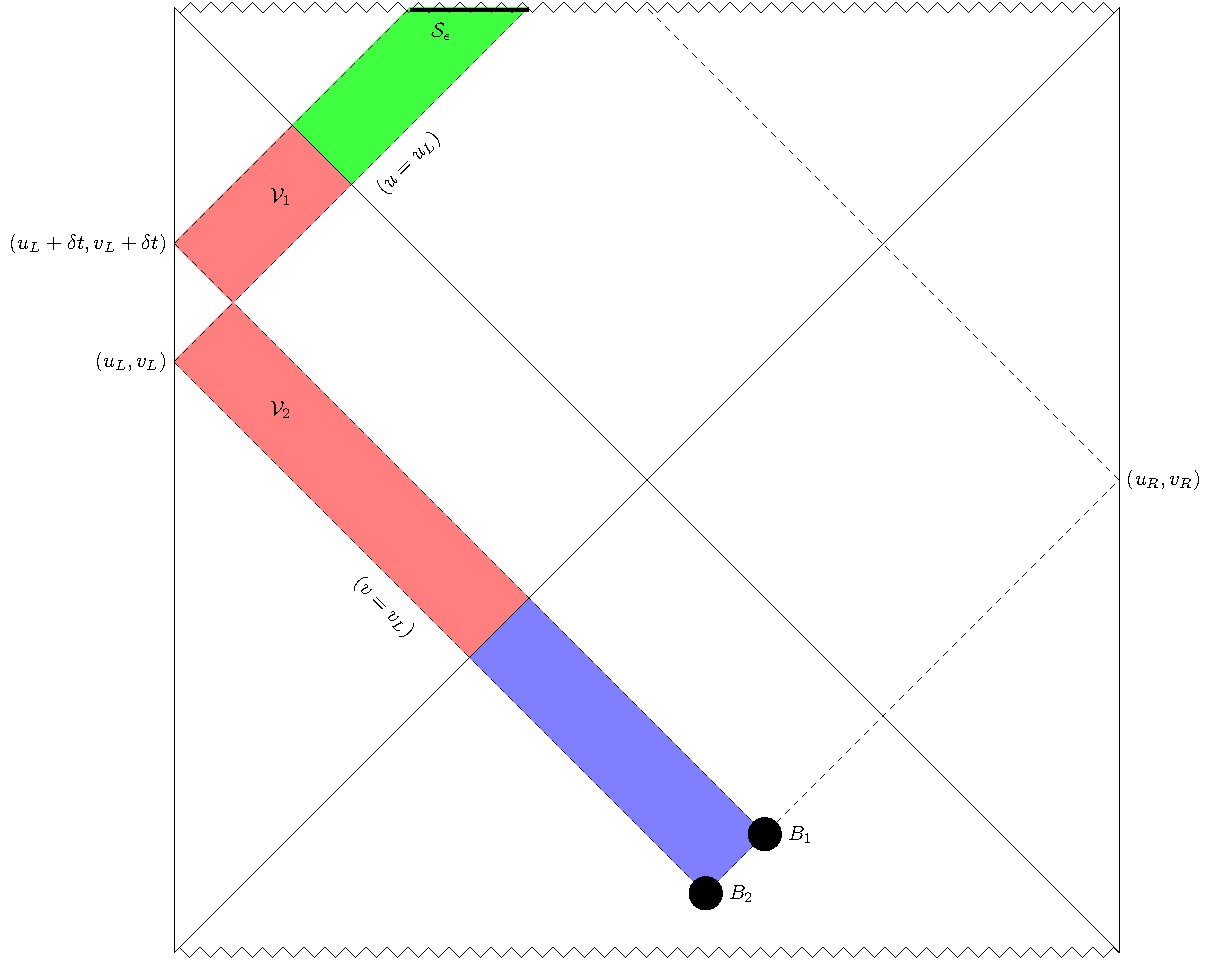
\includegraphics[scale=0.4]{WDWRateOfChange.pdf}   
    
    \end{center}
    \caption{Regions which contribute to rate of change}
    \label{fig:WDWSchw}
\end{figure}
}

\end{minipage}
}

\end{frame}
	
	\subsubsection{AdS-Kerr and AdS-RN}
	
\begin{frame}
\frametitle{CA for AdS-Ker}

\onslide<1->{
\begin{minipage}[t]{0.55\linewidth}

\begin{itemize}

\item \onslide<2->{Note that we now have a separate temperature, entropy, and thermodynamic volume for the inner and outer horizon.} 

\hfill

\item \onslide<3->{The corners labeled $B_1$ and $B_2$ tend towards the outer horizon in the late time limit and give a contribution of $T_+ S_+ \delta t$.} 

\hfill

\item \onslide<4->{The corners labeled $B_3$ and $B_4$ tend towards the inner horizon in the late time limit and give a contribution of $T_- S_- \delta t$.}

\hfill

\item \onslide<5->{Bulk term is proportional to $P(V^{+}_{th} - V^{-}_{th})$} 

\hfill

\item \onslide<6>{Similar result for AdS-RN} 
 
\end{itemize}

\end{minipage}\hfill
%
\begin{minipage}[t]{0.45\linewidth}

\begin{figure}
    \begin{center}
    
        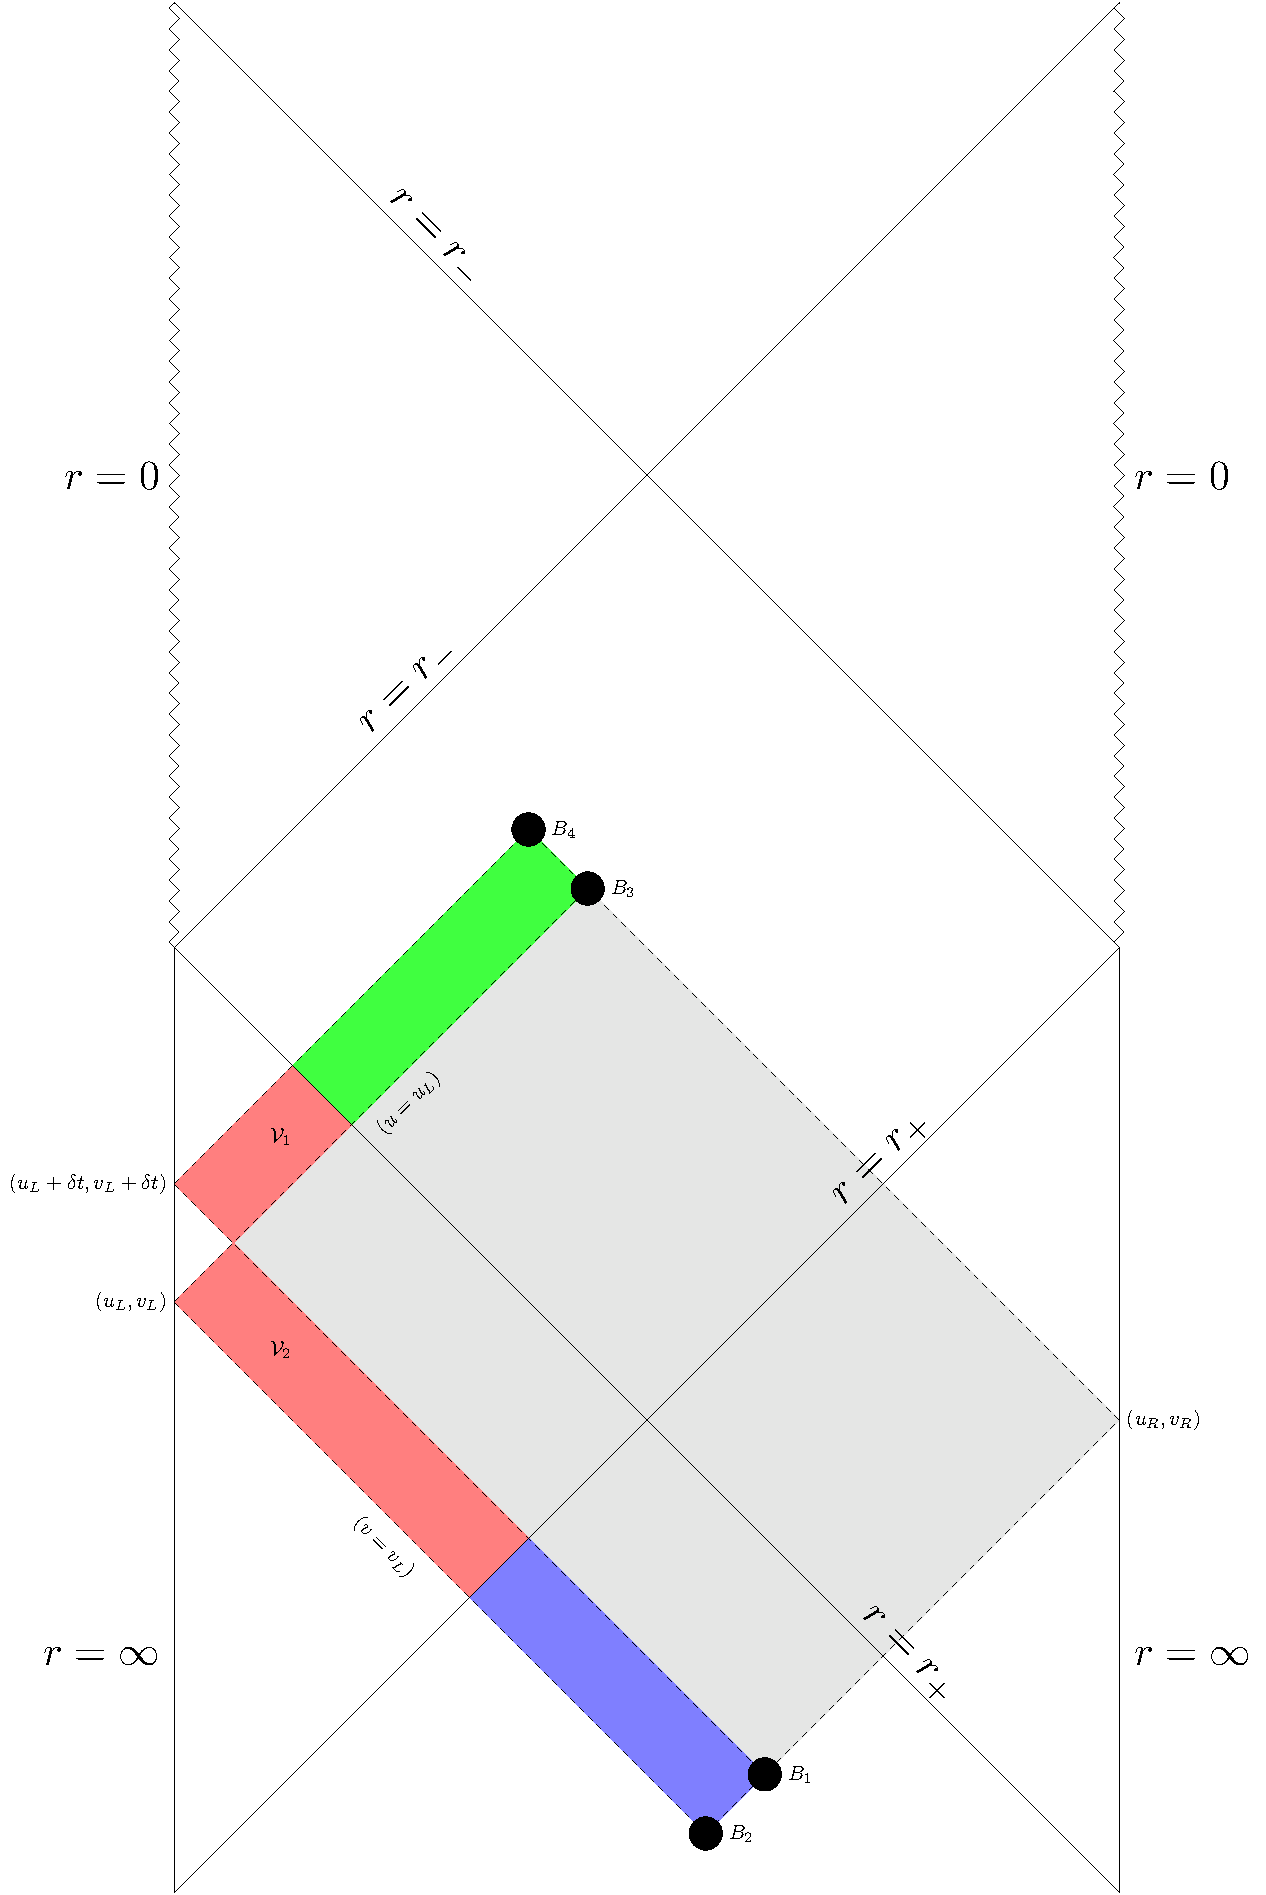
\includegraphics[scale=0.2]{WDWRN.pdf}   
    
    \end{center}
    \caption{Regions which contribute to rate of change}
    \label{fig:WDWRN}
\end{figure}
}

\end{minipage}

\end{frame}
	
\subsection{Complexity = Spacetime Volume?}


\begin{frame}
\frametitle{Complexity = Spacetime Volume}

\begin{itemize}

\item \onslide<1->{As we have seen, in vacuum spacetimes, where the on-shell Einstein-Hilbert action is proportional to the spacetime volume, the late time rate of change of the action of the WDW patch takes the form 
\begin{equation}
\frac{d}{dt} I_{WDW}|_{t\rightarrow \infty} \propto P (V^+_{th} - V^-_{th}).
\end{equation}
}

\hfill

\item \onslide<2->{This suggests perhaps we could make an alternative holographic complexity proposal such that $P V_{th}$ has the interpretation of being the asymptotic complexification rate, up to a factor of proportional to $\frac{1}{\hbar}$ }

\hfill

\item \onslide<3->{In fact, my co-authors and I proposed that perhaps the circuit complexity of the boundary state is dual to $\frac{P}{\hbar}$ times the spacetime volume of the relevant WDW patch }

\hfill

\item \onslide<4>{We termed this 'complexity = spacetime volume' or CV2.0}

\end{itemize}

\end{frame}


\begin{frame}
\frametitle{CA vs CV2.0}

\begin{itemize}

\item \onslide<1->{In most relevant respects, CV2.0 behaves qualitatively like CA or CV.}

\hfill

\item \onslide<2->{This is good because it means that all the reasons for suspecting complexity = volume or action are also relevant to CV2.0.}

\hfill


\item \onslide<3->{Like CA, CV2.0 shows indefinite linear growth at late time.}

\hfill

\item \onslide<4->{It also has the right behavior in shockwave geometries}

\hfill

\item \onslide<5>{One thing that does distinguish them (to some extent) is the Lloyd bound }

\end{itemize}

\end{frame}


\begin{frame}
\frametitle{The Lloyd Bound}

\begin{itemize}

\item \onslide<1->{The Lloyd bound comes from the Margolus-Levitin theorem.}

\hfill

\item \onslide<2->{Margolus and Levitin, 1997 \cite{Margolus:1997ih}: Given a quantum state $\ket{\psi}$ with average energy $E = \expval{H}_\psi$, the time it takes to evolve to an orthogonal state is bounded by 
\begin{equation}
t_{\perp} \geq \frac{h}{4 E}
\end{equation}
}

\hfill

\item \onslide<3->{If the states corresponding to the WDW patches for $t$ and $t+\Delta t$ are orthogonal, then this implies
\begin{eqnarray}
\dot{\mathcal{C}} \approx \frac{N}{\Delta t} \leq \frac{2 E N}{\pi \hbar}
\end{eqnarray}
}

\hfill

\item \onslide<4->{Where $N$ is the complexity of evolving for time $\Delta t$}

\hfill

\item \onslide<5>{If we take $\Delta t$ to be the smallest time interval such that these states are orthogonal, and take the corresponding $N$ to be $1$, we get the Lloyd bound \cite{Lloyd}:
\begin{equation}
\dot{\mathcal{C}} \leq \frac{2 E}{\pi \hbar}
\end{equation}
}

\end{itemize}

\end{frame}

\begin{frame}
\frametitle{CA vs CV2.0: The Lloyd Bound}

\begin{itemize}

\item \onslide<2->{ exact results for AdS-RN with $\mu \leq 1$:}

\hfill

\begin{itemize}

\item \onslide<3->{CA: Always violates the Lloyd bound for $\mu \leq 1$ and $d\geq 4$.}

\hfill

\item \onslide<4->{CV2.0: Never violates the Lloyd bound for $\mu \leq 1$ and in $d=4$ or $d=5$.}

\hfill

\end{itemize}

\item \onslide<5->{ Near extremal results for AdS-RN with $\mu \geq 1$:}

\hfill

\begin{itemize}

\item \onslide<6->{CA and CV2.0: $\dot{\mathcal{C}} \sim \mathcal{O}\left(\delta M\right)$ ($\delta M = M - M_{\text{extremal}}$)}

\hfill

\item \onslide<7->{Lloyd Bound: $\dot{\mathcal{C}}_{\max} \sim \mathcal{O}\left(\delta M^2\right)$}

\hfill

\item \onslide<8->{$\Rightarrow$ both proposals must violate Lloyd bound near extremality.}

\end{itemize}

\end{itemize}

\end{frame}

\begin{frame}
\frametitle{Part II recap}

\begin{itemize}

\item \onslide<1->{We may extend the usual black hole thermodynamics by allowing variations in the cosmological constant.}

\hfill

\item \onslide<2->{This leads to a term in the first law that can be understood as a pressure-volume work term.}

\hfill

\item \onslide<3->{However, the resulting volume ($V_{th}$) is not a geometric volume.}

\hfill

\item \onslide<4->{When the late time rate of complexity increase is computed according to CA, the bulk contribution is proportional to $P V_{th}$}

\hfill

\item \onslide<5->{We can propose an alternative to CA, namely CV2.0, for which $P V_{th}$ is the only contribution.}

\hfill

\item \onslide<6->{Most of the arguments in favor of CA also apply to CV2.0.}

\hfill

\item \onslide<7->{Neither CA nor CV2.0 always obeys the Lloyd bound, though CV2.0 seems to obey it more often.}

\hfill

\item \onslide<8>{Under either of CA or CV2.0, there seems to be a connection between extended thermodynamics and the rate of increase of complexity}

\end{itemize}

\end{frame}

\section{Holographic Subregion Complexity and Purification Complexity}\begin{frame}
\sectionpage
	\begin{center}
		Based on 1811.10650\\
		Work with Elena C\'aceres, Stefan Eccles, and Willy Fischler
	\end{center}
\end{frame}

%
%\begin{frame}
%
%This is a beamer frame
%
%\end{frame}

\subsection{Subregion complexity}


\begin{frame}
\frametitle{Subregion complexity}

\begin{minipage}[t]{0.48\linewidth}

\begin{itemize}

\item \onslide<1->{The bulk side of the various holographic complexity proposals (CA, CV, CV2.0) can all be easily extended to a submanifold of some geodesically complete space}

\hfill

\item \onslide<2->{In particular, one can extend each of these to any entanglement wedge in an asymptotically AdS spacetime}

\hfill

\item \onslide<5->{What are these bulk quantities dual to?}

\hfill

\item \onslide<6->{It seems natural to conjecture that these quantities are dual to some notion of complexity on a subsystem}

\hfill

\item \onslide<7>{How does one define circuit complexity on a mixed state?}

\end{itemize}

\end{minipage}
%
\hfill
%
\begin{minipage}[t]{0.48\linewidth}

\only<1-2>{
\begin{figure}
    \begin{center}
    
        \includegraphics[scale=0.35]{2sidedBH}    
    
    \end{center}
    \caption{Two-sided black hole}
    \label{fig:Two-sided black hole}
\end{figure}
}

\only<3>{
\begin{figure}
    \begin{center}
    
        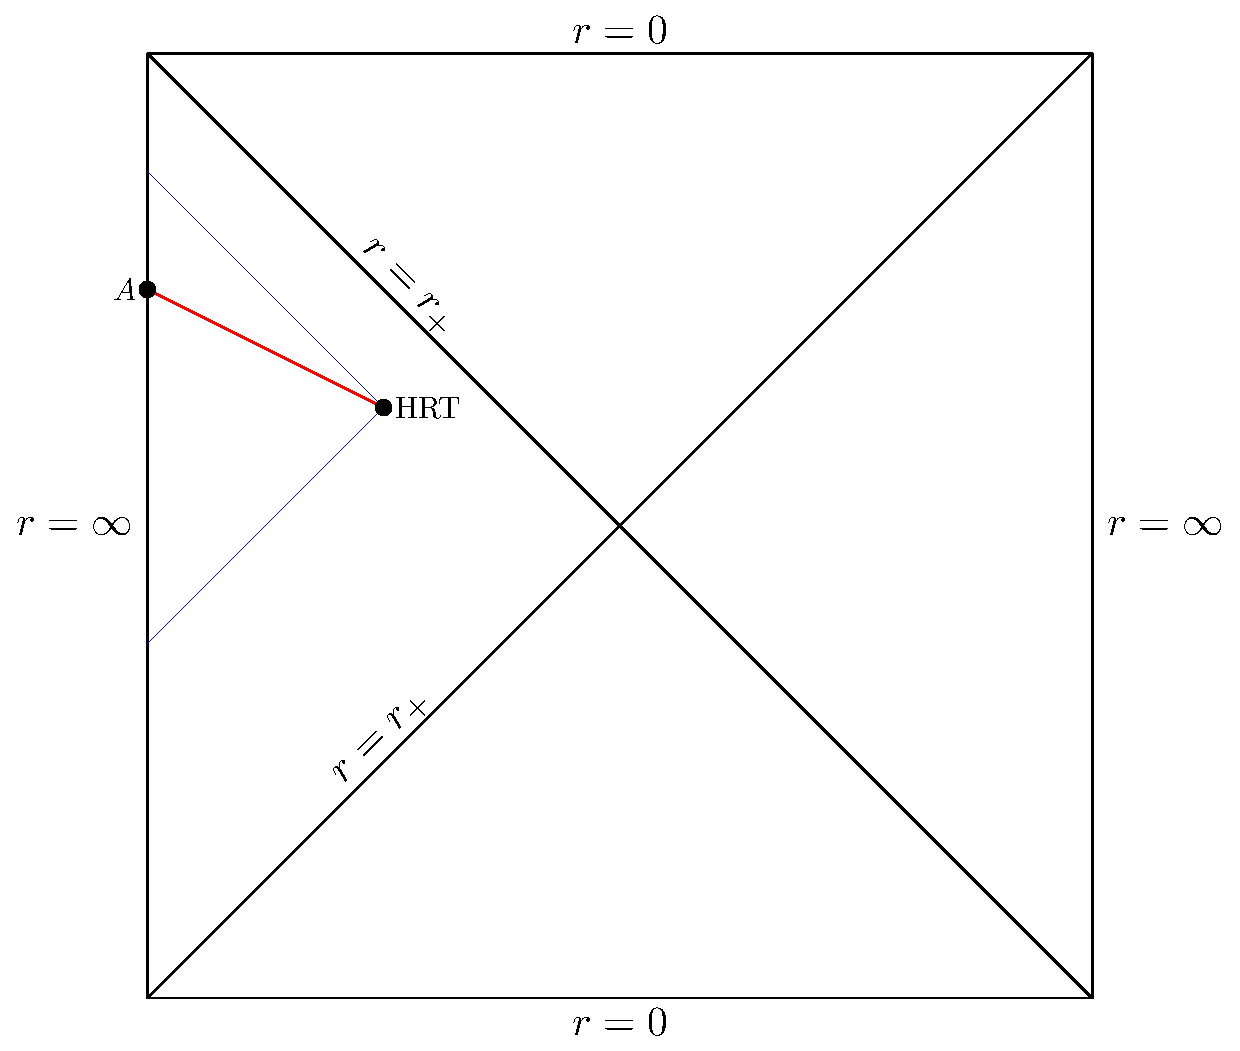
\includegraphics[scale=0.35]{subregion_complexity_CV}    
    
    \end{center}
    \caption{Subregion complexity: CV}
    \label{fig:adscft}
\end{figure}
}

\only<4>{
\begin{figure}
    \begin{center}
    
        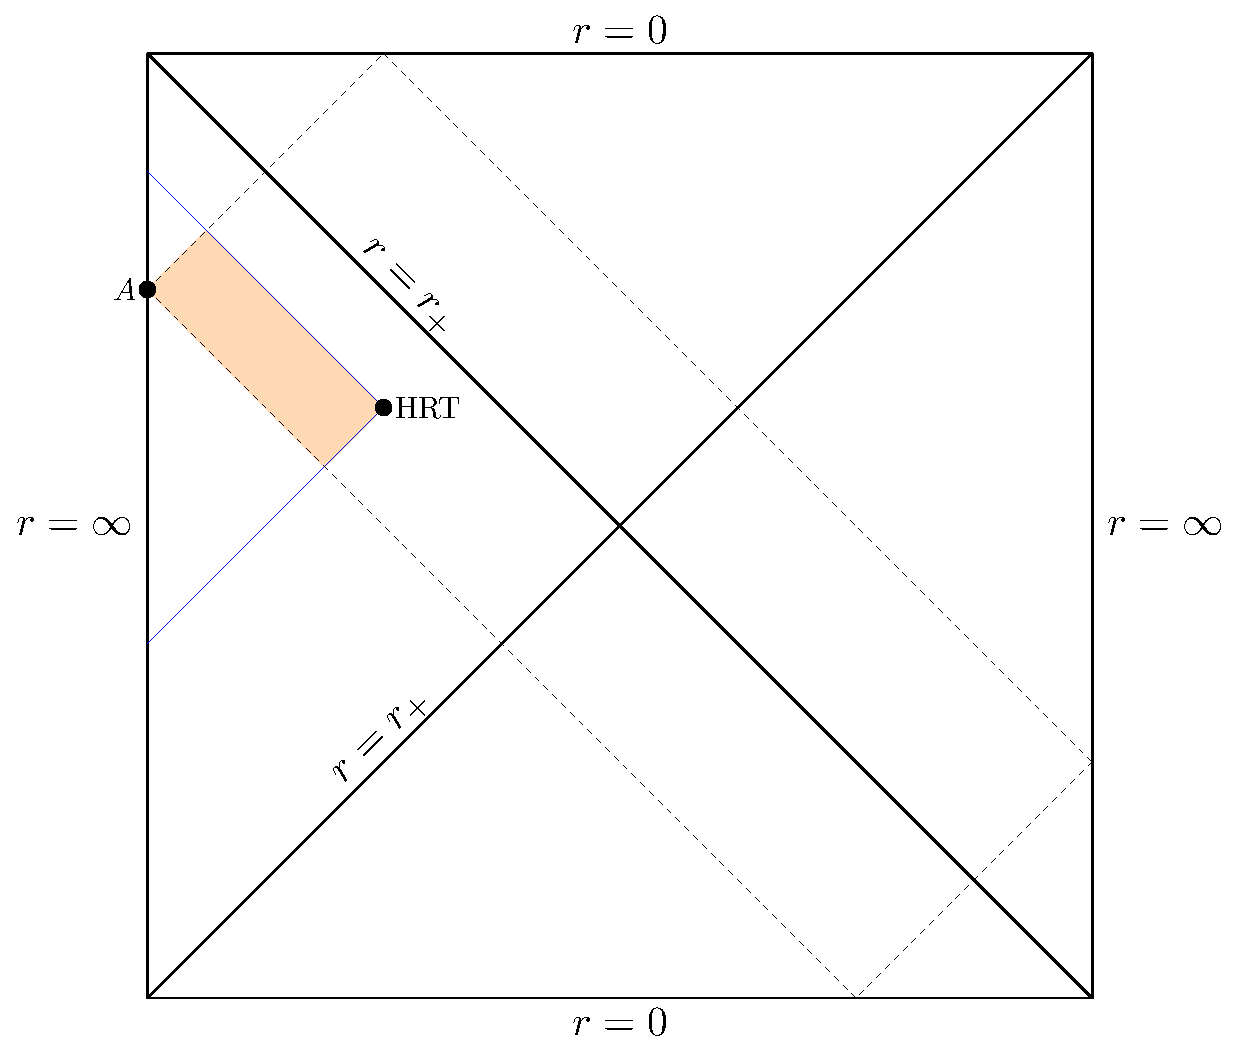
\includegraphics[scale=0.35]{subregion_complexity_WDW}    
    
    \end{center}
    \caption{Subregion complexity: CA and CV2.0}
\end{figure}
}

\only<5->{
\begin{figure}
    \begin{center}
    
        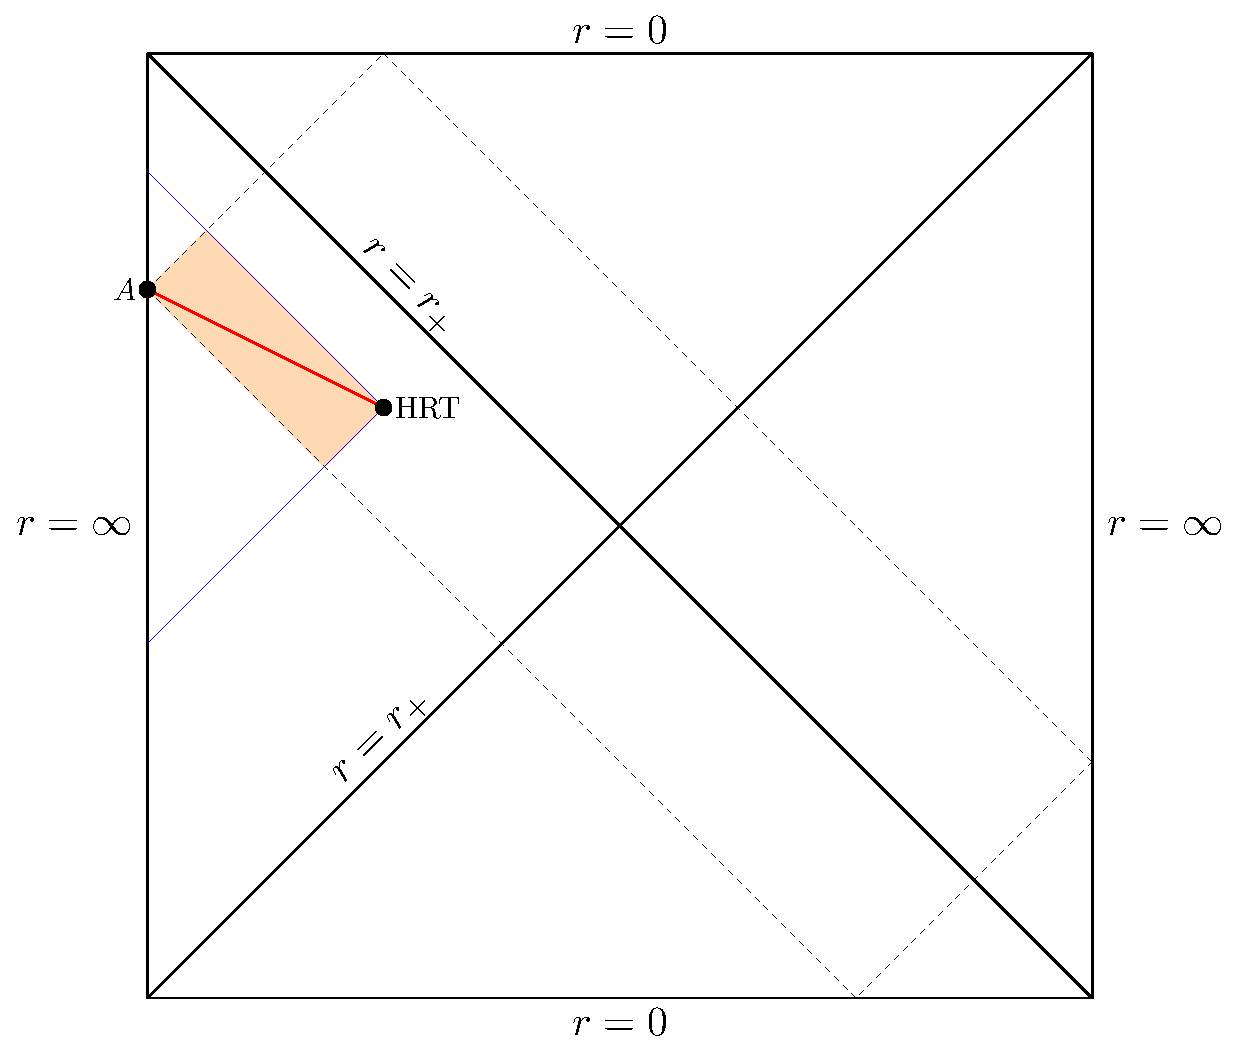
\includegraphics[scale=0.35]{subregion_complexity}    
    
    \end{center}
    \caption{Subregion complexity}
\end{figure}
}

\end{minipage}


\end{frame}


\begin{frame}
\frametitle{Purification complexity}

\begin{itemize}

\item \onslide<1->{There are actually many different possible extensions to the notion of circuit complexity to a mixed state (such as the state on a subregion)}

\hfill

\item \onslide<2->{We will focuse on the {\it purification complexity}}

\hfill


\item \onslide<3->{
Given a mixed state $\rho$ on system $A$, a purification of $\rho$ on a system $B = A \otimes \bar{A}$ is a pure state $\ket{\psi}$ such that $\tr_{\bar{A}} \left( \ket{\psi} \bra{\psi} \right) = \rho$ 
}

\hfill

\item \onslide<4->{
The purification complexity of the mixed state $\rho$ is then the minimum complexity out of the complexities of all possible purifications of $\rho$
}

\hfill

\item \onslide<5>{
I.e.
\begin{equation}
\mathcal{C}_{\text{purification}} (\rho) = \min_{\ket{\psi} : \psi \text{ purifies } \rho} \mathcal{C}(\ket{\psi})
\end{equation}
}

\end{itemize}

\end{frame}

\subsection{A consistency test for subregion complexity = purification complexity}


\begin{frame}
\frametitle{A consistency test}

\begin{itemize}

\item \onslide<1->{
We would like to test the conjecture that subregion complexity (as defined by CA, CV, or CV2.0) on an entanglement wedge is dual to the purification complexity of the dual mixed state.
}

\hfill

\item \onslide<2->{
One obstacle to testing this is that complexity is not that well understood in QFT, and computing purification complexity is actually very hard.
}

\hfill

\item \onslide<3->{
However, there seems to be a consistency test that is easy to do.
}

\hfill

\item \onslide<4->{
For any entanglement wedge contained in a geodesically complete holographic spacetime, the state dual to the whole geometry should be a purification of the state on the subsystem which defines the entanglement wedge.
}

\hfill

\item \onslide<5->{
'subregion complexity = purification complexity' thus predicts that the subregion complexity computed by applying CA/CV/CV2.0 to an entanglement wedge should always be smaller than the result of applying the relevant conjecture to the whole geometry.
}

\hfill

\item \onslide<6>{
We can actually get a holographic bound on purification complexity by considering different holographic purifications.
}

\end{itemize}

\end{frame}


\begin{frame}
\frametitle{Different holographic purifications}



\begin{minipage}[t]{0.48\linewidth}

\hfill

\begin{itemize}

\item \onslide<1->{Consdider left side of 2-sided BTZ BH (at time $t_L$)
}

\hfill

\item \onslide<2->{Different choices of $t_R$ lead to different purifications.
}

\hfill

\item \onslide<3->{Optimal is $t_R = -t_L$
}

\hfill

\item \onslide<4->{2-sided BTZ is one of many quotients of pure AdS}

\hfill

\item \onslide<5->{Can consider $n$-sided genus $g$ black holes.}

\hfill

\item \onslide<6->{What about changing the right cutoff?.}

\hfill

\item \onslide<9>{If this makes sense, the optimum is when cutoff hugs the horizon (For CV and CV2.0, CA less clear).}

\end{itemize}

\end{minipage}
%
\hfill
%
\begin{minipage}[t]{0.48\linewidth}

\only<1>{
\begin{figure}
    \begin{center}
    
        
\includegraphics[scale=0.4]{WDW2}    
    
    \end{center}
    \caption{Holographic Purifications}
    \label{fig:EofP}
\end{figure}
}

\only<2>{
\begin{figure}
    \begin{center}
    
        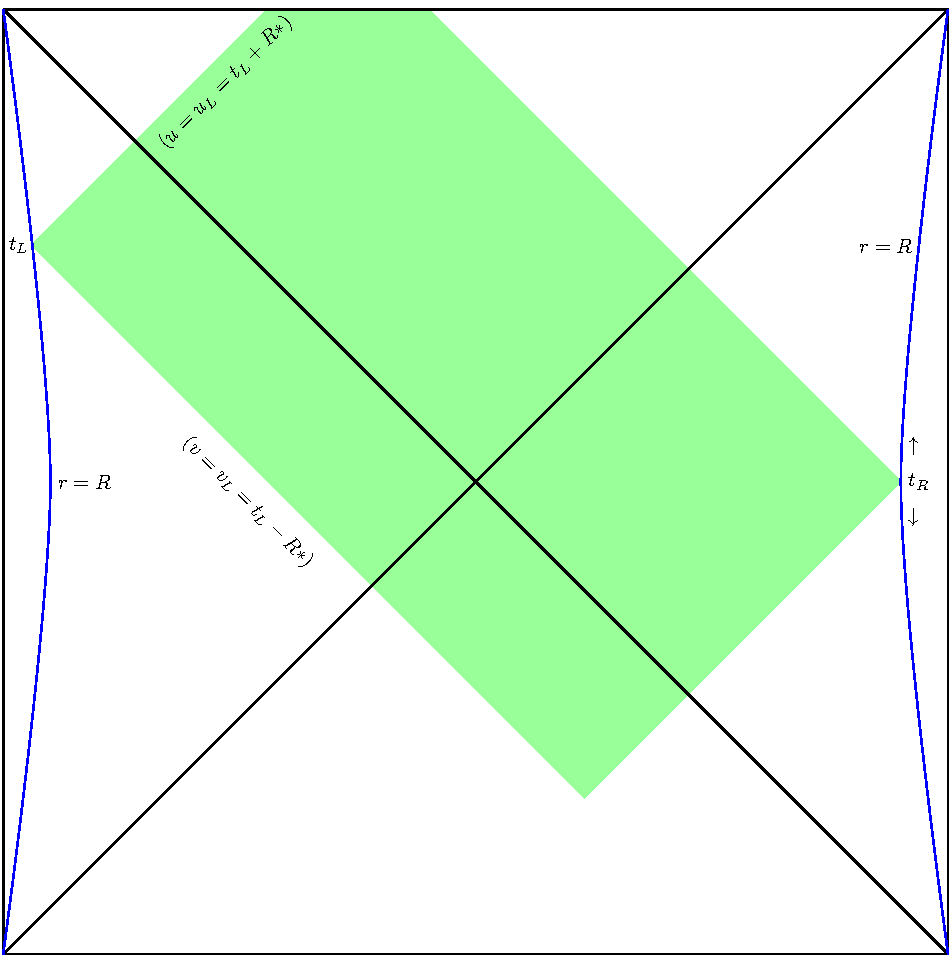
\includegraphics[scale=0.4]{WDWUpDown}    
    
    \end{center}
    \caption{Holographic Purifications}
    \label{fig:EofP}
\end{figure}
}

\only<3-5>{
\begin{figure}
    \begin{center}
    
        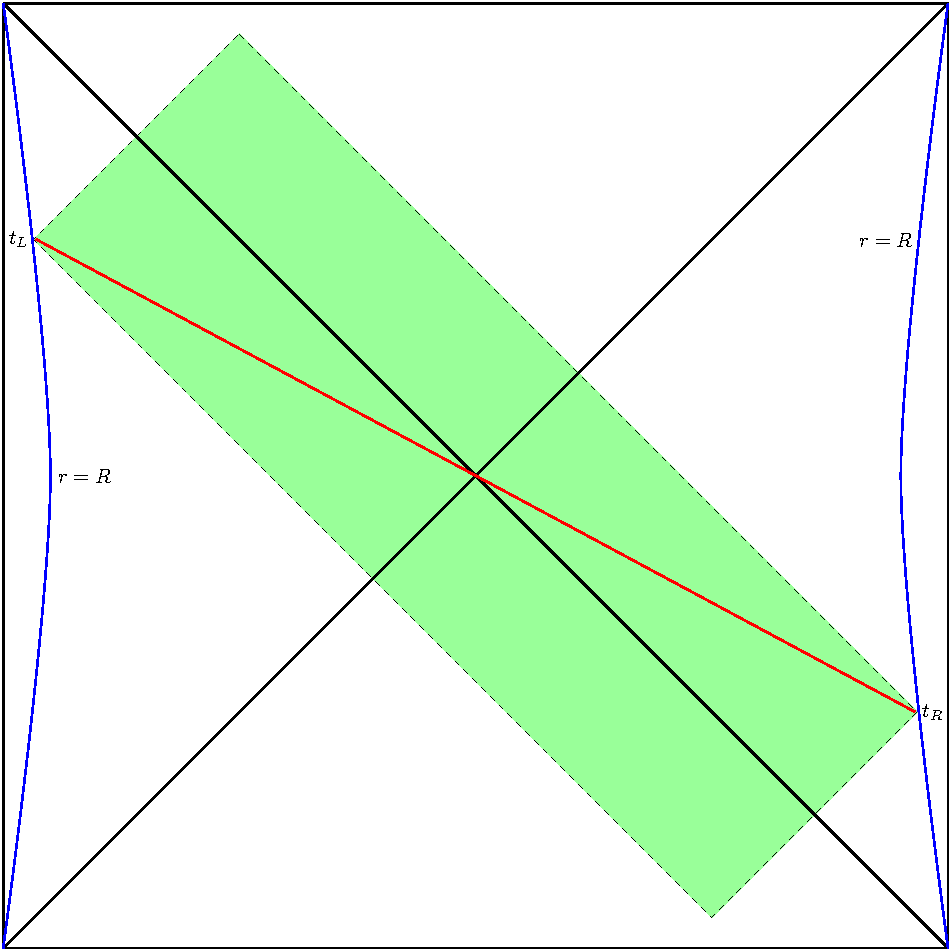
\includegraphics[scale=0.4]{WDWSym}    
    
    \end{center}
    \caption{Holographic Purifications}
    \label{fig:EofP}
\end{figure}
}

\only<6>{
\begin{figure}
    \begin{center}
    
        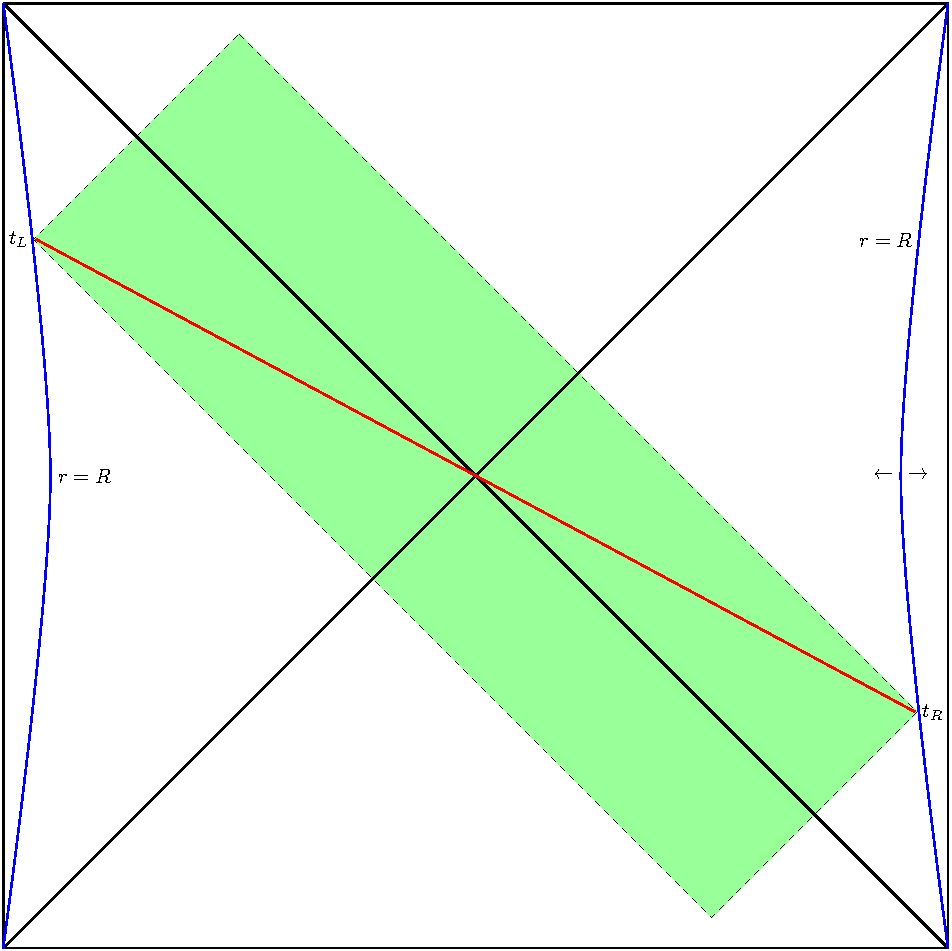
\includegraphics[scale=0.4]{WDWLeftRight}    
    
    \end{center}
    \caption{Holographic Purifications}
    \label{fig:EofP}
\end{figure}
}

\only<7>{
\begin{figure}
    \begin{center}
    
        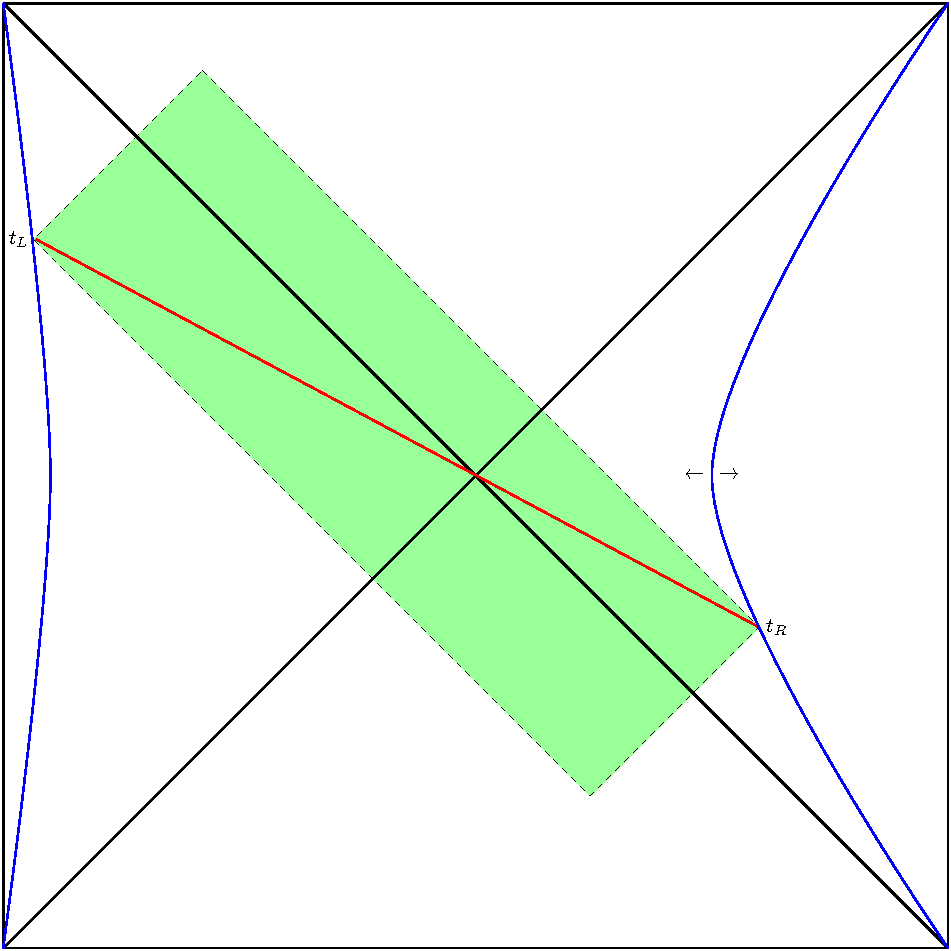
\includegraphics[scale=0.4]{WDWSmallRightCutoff0}    
    
    \end{center}
    \caption{Holographic Purifications}
    \label{fig:EofP}
\end{figure}
}

\only<8->{
\begin{figure}
    \begin{center}
    
        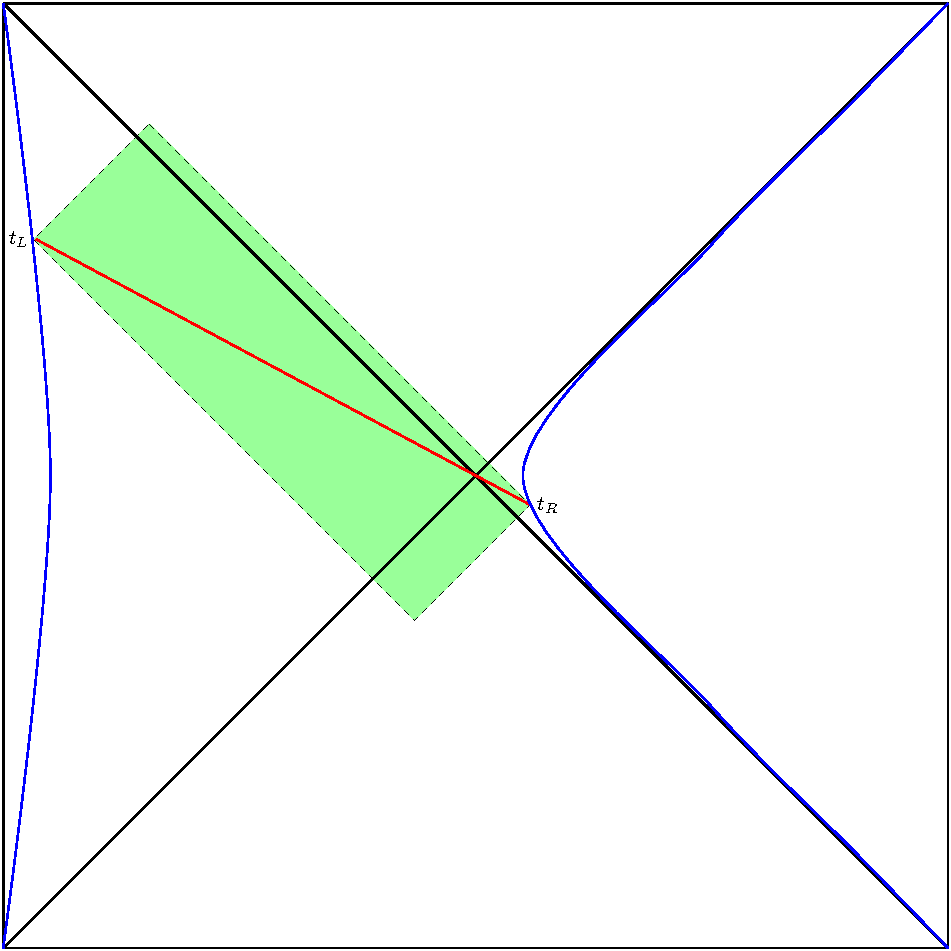
\includegraphics[scale=0.4]{WDWSmallRightCutoff}    
    
    \end{center}
    \caption{Holographic Purifications}
    \label{fig:EofP}
\end{figure}
}

\end{minipage}

\end{frame}



\begin{frame}
\frametitle{CV and CV2.0: Superadditivity}

\onslide<1->{
\begin{minipage}[t]{0.48\linewidth}

\begin{itemize}

\item \onslide<1->{Assuming either CV or CV2.0, we can easily prove that for two disjoint subregions $A$ and $B$,
\begin{equation}
\mathcal{C}(A) + \mathcal{C}(B) \leq \mathcal{C}(AB).
\end{equation}
}

\item \onslide<2->{CV2.0: Obvious because spacetime volume is additive and positive definite }

\hfill

\item \onslide<3->{CV, where $A\cup B$ is full system: Obvious because spatial volume is additive and positive definite }

\hfill

\item \onslide<4->{$\Rightarrow$ CV and CV2.0 can't fail propsed test}

\hfill

\item \onslide<5->{CV general case: All we need is a spatial slice to 'bridge the gap'}

\hfill

\item \onslide<6>{No such proof for CA: action is additive but not positive definite}

\end{itemize}

\end{minipage}
%
\hfill
%
\begin{minipage}[t]{0.48\linewidth}

\only<2>{
\begin{figure}
    \begin{center}
    
        \includegraphics[scale=1.2]{img/WDW_SSA}    
    
    \end{center}
    \caption{Superadditivity for CV2.0}
    \label{fig:adscft}
\end{figure}
}

\only<3-4>{
\begin{figure}
    \begin{center}
    
        \includegraphics[scale=1.2]{img/SA_BH2}    
    
    \end{center}
    \caption{Superadditivity for CV}
    \label{fig:adscft}
\end{figure}
}

\only<5->{
\begin{figure}
    \begin{center}
    
        \includegraphics[scale=1]{img/SA_bridge2}    
    
    \end{center}
    \caption{Superadditivity for CV}
    \label{fig:adscft}
\end{figure}
}

\end{minipage}
}

\end{frame}


\begin{frame}
\frametitle{Subregion vs purification complexity under CA}

\begin{itemize}

\item \onslide<1->{Because the action is additive but not positive definite, it can happen that the subregion complexity, as computed by CA, is larger than the full complexity.}

\hfill

\item \onslide<2->{There are actually several examples where this happens}

\hfill

\begin{itemize}

\item \onslide<3->{Black holes with non-trivial genus (Fu et al. \cite{Fu:2018kcp})}

\hfill

\item \onslide<4->{Ordinary two-sided black holes, for certain values of cutoff and arbitrary length scale}

\hfill

\item \onslide<5->{Poincar\'e patch quotiented by a spatial translation, once again for certain values of the cutoff or arbitrary length scale}

\hfill

\end{itemize}

\item \onslide<6->{It is tempting to say that these examples show that the CA version of subregion complexity = purification complexity is inconsistent}

\hfill

\item \onslide<7>{However, one might also argue that the parameter choices involved are for some reason not allowed}

\end{itemize}

\end{frame}

\subsection{Analogy with entanglement of purification}


\begin{frame}
\frametitle{Does subregion complexity = purification complexity?}

\begin{minipage}[t]{0.48\linewidth}

\begin{itemize}

\item \onslide<1->{CV and CV2.0: Pretty clear, if changing cutoff is okay.}

\hfill

\item \onslide<2->{Small cutoff $\rightarrow$ spacetime volume and volume approach subregion values}

\hfill

\item \onslide<3->{Is this okay though?}

\hfill

\item \onslide<4>{Seems similar to what is going on with {\it entanglement of purification}}

\end{itemize}

\end{minipage}
%
\hfill
%
\begin{minipage}[t]{0.48\linewidth}

\only<1->{
\begin{figure}
    \begin{center}
    
        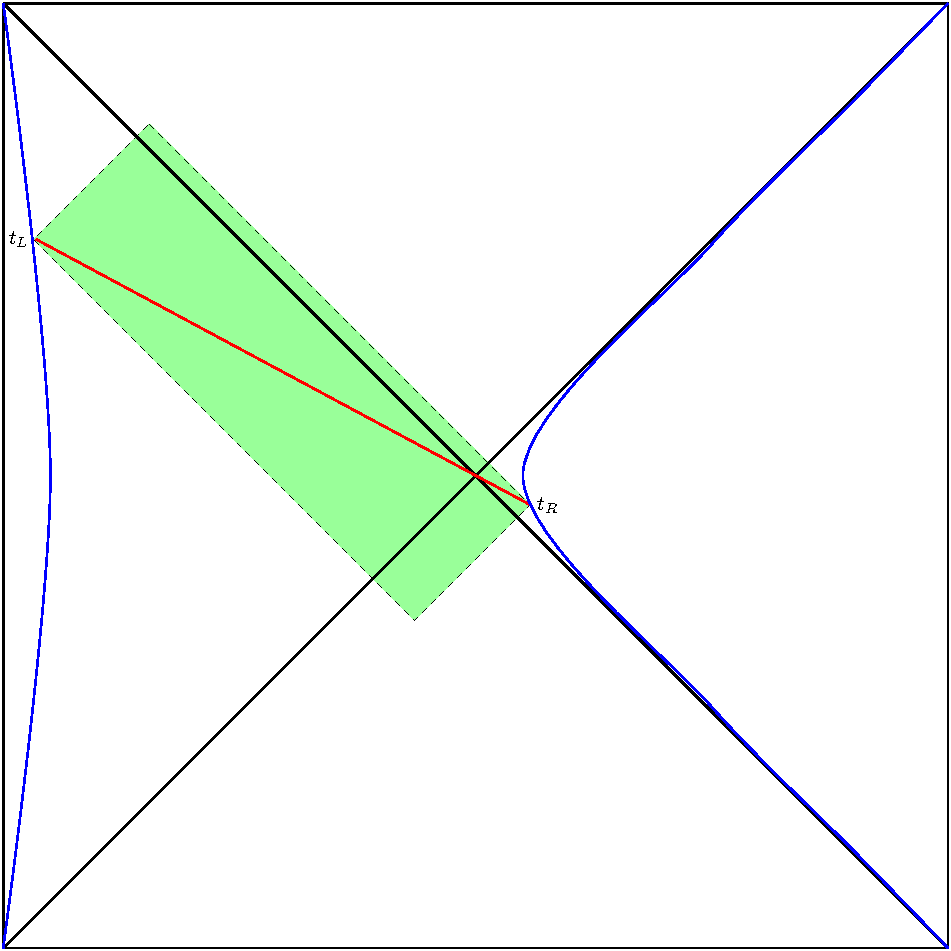
\includegraphics[scale=0.4]{WDWSmallRightCutoff}    
    
    \end{center}
    \caption{Small cutoff again}
    \label{fig:EofP}
\end{figure}
}

\end{minipage}

\end{frame}


\begin{frame}
\frametitle{Entanlgement of Purification}

\begin{minipage}[t]{0.48\linewidth}

\hfill

\begin{itemize}

\item \onslide<1->{Definition: 
\begin{eqnarray}
S^P(\rho_{AB}) = \min_{\ket{\psi}_{A\bar{A}B\bar{B}}} S(\rho_{A\bar{A}})\\
\rho_{AB} = \tr_{\bar{A}\bar{B}} \left(\ket{\psi}\bra{\psi}\right)\\
\rho_{A\bar{A}} = \tr_{B\bar{B}} \left(\ket{\psi}\bra{\psi}\right)
\end{eqnarray}
}

\item \onslide<2->{Holographic proposal \cite{Takayanagi:2017knl, Nguyen:2017yqw, Bao:2017nhh}:
}

\hfill

\begin{itemize}

\item \onslide<3->{Zero mutual info: zero}

\hfill

\item \onslide<4->{Non-zero mutual info: Area of minimal surface dividing A from B (in entanglement wedge)}

\hfill

\item \onslide<5->{Purifying d.o.fs thought of as living on RT surface}

\hfill

\item \onslide<6>{Perhaps this can also be understood in terms of a minimization over cutoffs?}


\end{itemize}

\end{itemize}

\end{minipage}
%
\hfill
%
\begin{minipage}[t]{0.48\linewidth}

\only<1-5>{
\begin{figure}
    \begin{center}
    
        \includegraphics[scale=1.2]{img/EofP}    
    
    \end{center}
    \caption{Holographic Entanglement of Purification}
    \label{fig:EofP}
\end{figure}
}

\only<6>{
\begin{figure}
    \begin{center}
    
        \includegraphics[scale=1.2]{img/EofP2}    
    
    \end{center}
    \caption{Holographic Entanglement of Purification}
    \label{fig:EofP}
\end{figure}
}

\end{minipage}

\end{frame}


\begin{frame}
\frametitle{Part III recap}

\begin{itemize}

\item \onslide<1->{CA, CV, and CV2.0 can all be easily extended to be applied on an entanglement wedge.}

\hfill

\item \onslide<2->{It is natural to think that if the normal versions of these conjectures are true, then the entanglement wedge version corresponds to a notion of complexity for the reduced state on the subregion.}

\hfill

\item \onslide<3->{One such notion is the purification complexity.}

\hfill

\item \onslide<4->{If subregion complexity = purification complexity, then the subregion complexity computed for an entanglement wedge must be smaller than the complexity computed for the geodesically complete space.}

\hfill

\item \onslide<5->{CV and CV2.0 always obey this property.}

\hfill

\item \onslide<6->{For CA there are counterexamples.}

\hfill

\item \onslide<7>{If we are allowed to change cutoff (for complimentary region), it is clear subregion complexity and purification complexity coincide for CV and CV2.0.}

\end{itemize}

\end{frame}

\section{Conclusion and Discussion}

\begin{frame}
\frametitle{Conclusion and Discussion}

\begin{itemize}

\item \onslide<1->{We have discussed \ldots}

\hfill

	\begin{itemize}

	\item \onslide<2->{\ldots the holographic complexity conjectures (CA, CV, and CV2.0).}

\hfill

	\item \onslide<3->{\ldots extended black hole thermodynamics and a possible connection to complexity.}

\hfill

	\item \onslide<4->{\ldots subregion complexity and its possible duality with purification complexity.}

\hfill

	\end{itemize}

\item \onslide<5->{Further questions:}

\hfill

	\begin{itemize}

	\item \onslide<6->{What is the interpretation of $V_{th}$ in non-AdS spacetimes (e.g. dS)? }

\hfill

	\item \onslide<7->{How should we understand the difficulties with (subregion) CA?}

\hfill

	\item \onslide<8>{Can an analog of CA/CV/CV2.0 be defined for tensor networks? For quantum error-correcting codes?}

	\end{itemize}

\end{itemize}

\end{frame}


\begin{frame}
\frametitle{References}
{\tiny
\bibliographystyle{JHEP} %JHEP.bst
\footnotesize\bibliography{content/diss}
}
\end{frame}


\begin{frame}
\frametitle{Behind the BH Horizon}

\onslide<1->{
I stated before that a black hole geometry is dual to a thermal state. Strictly speaking, it is geometry outside the horizon that is dual to a thermal state. 

\begin{minipage}[t]{0.55\linewidth}

\begin{itemize}

\item \onslide<2->{The (geodesically) complete geometry is a two-sided black hole geometry}

\item \onslide<3->{This geometry has two boundaries, with a CFT  on each boundary. The Hilbert space is given by $\mathcal{H} = \mathcal{H}_L \otimes \mathcal{H}_R$ }

\item \onslide<4->{The state dual to this configuration is a purification of the thermal state known as the thermofield double state: 

$$\psi = \displaystyle\sum_n e^{- \beta E_n /2} \ket{E_n}_L \otimes \ket{E_n}_R$$ }

\item \onslide<5->{Outside of horizon geometry corresponds in some sense to the entanglement structure of the thermal state.}

\item \onslide<6>{What about the geometry behind the horizon?}

\end{itemize}

\end{minipage}\hfill
%
\begin{minipage}[t]{0.44\linewidth}

\begin{figure}
    \begin{center}
    
        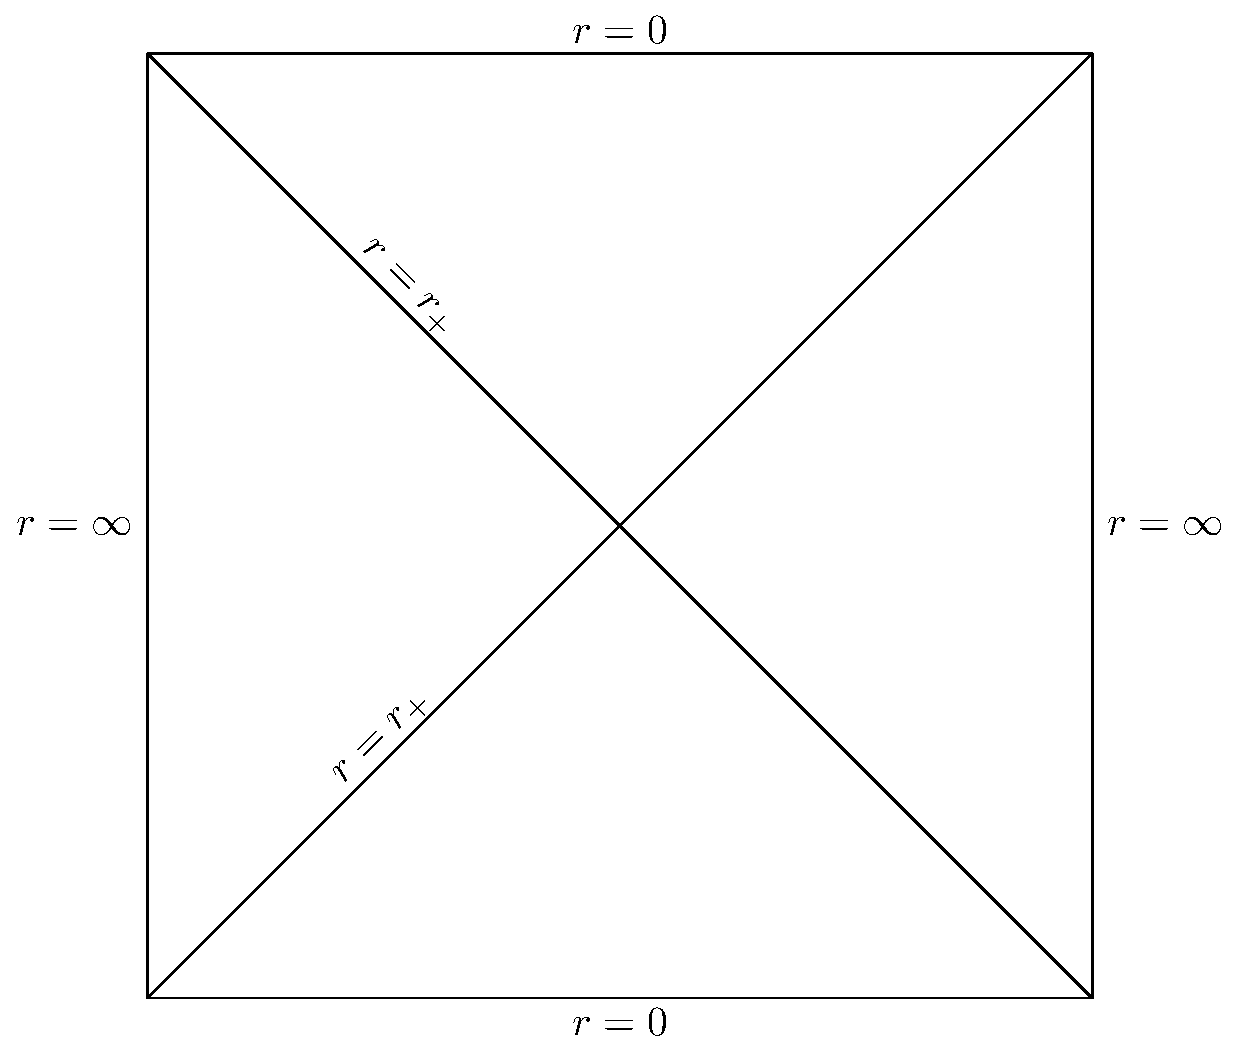
\includegraphics[scale=0.3]{2SidedBH}    
    
    \end{center}
    \caption{Two-sided black hole}
    \label{fig:2SidedBH}
\end{figure}

\end{minipage}
}

\end{frame}


\begin{frame}
\frametitle{Switchback effect}

One of the main pieces of evidence in favor of CA and CV comes from the switchback effect.

\hfill

\begin{itemize}

\item \onslide<2->{Consider the operator $U(-t)WU(t)$}

\hfill

\item \onslide<3->{What is its complexity?}

\hfill

	\begin{itemize}
	
	\item \onslide<4->{
	\begin{equation}
		\mathcal{C}\left(U(-t)WU(t) \right) \leq \mathcal{C}\left(U(-t) \right) + \mathcal{C}\left(W \right) + \mathcal{C}\left(U(t) \right)
	\end{equation}
	}

\hfill
	
	\item \onslide<5->{If $W$ is the identity, complexity is zero}

\hfill
	
	\item \onslide<6->{For small $W$, generically get linear growth for $t>t_{\text{sat}}$}

\hfill
	
	\end{itemize}

\item \onslide<7->{This type of operator is dual to shockwave insertions in AdS}

\item \onslide<8>{CA and CV exhibit the expected behavior when applied to these shockwave geometries}

\end{itemize}

\end{frame}

\begin{frame}
\frametitle{Complexity = Action}

Complexity = volume has a few unpleasant features.

\begin{itemize}

\item For example, in order to reproduce the correct boundary behavior, the volume must be multiplied by a non-universal length scale

\end{itemize}

One might seek an alternative proposal, which still captures something about the geometry behind the horizon, but which does not have these features. Such an alternative has been proposed by Susskind et al. \cite{Brown:2015bva, Brown:2015lvg}, and it goes by 'complexity = action.'

\begin{itemize}

\item According to complexity = action, the complexity is dual to the action of a so-called 'Wheeler-DeWitt' (WDW) patch.

\item Because this is an action, it can be nondimensionalized with some multiple of $\hbar$. 

\item A universal choice for this coefficient is consistent with the expected large temperature behavior. 

\item Also exhibits linear growth at late time etc.

\end{itemize}

\end{frame}


\end{document}
